\section{Introduction to Languages,IDE’s,Tools and Technologies used for Implementation}
	
\subsection{Technologies used}

\subsubsection{Firebase}

Firebase helps you build better mobile apps and grow your business.

Firebase is a mobile platform from Google offering a number of different features that you can pick ‘n mix from. Specifically, these features revolve around cloud services, allowing users to save and retrieve data to be accessed from any device or browser. This can be useful for such things as cloud messaging, hosting, crash reporting, notifications, analytics and even earning money through AdMob.

It works with Android apps, iOS apps and web apps and best of all: it’s free!

\begin{itemize}

\item \textbf{Setting up a project}

Before you can do anything with Firebase, you first need to create an account. You can do this over at firebase.google.com.

\begin{figure}[ht]
\centering
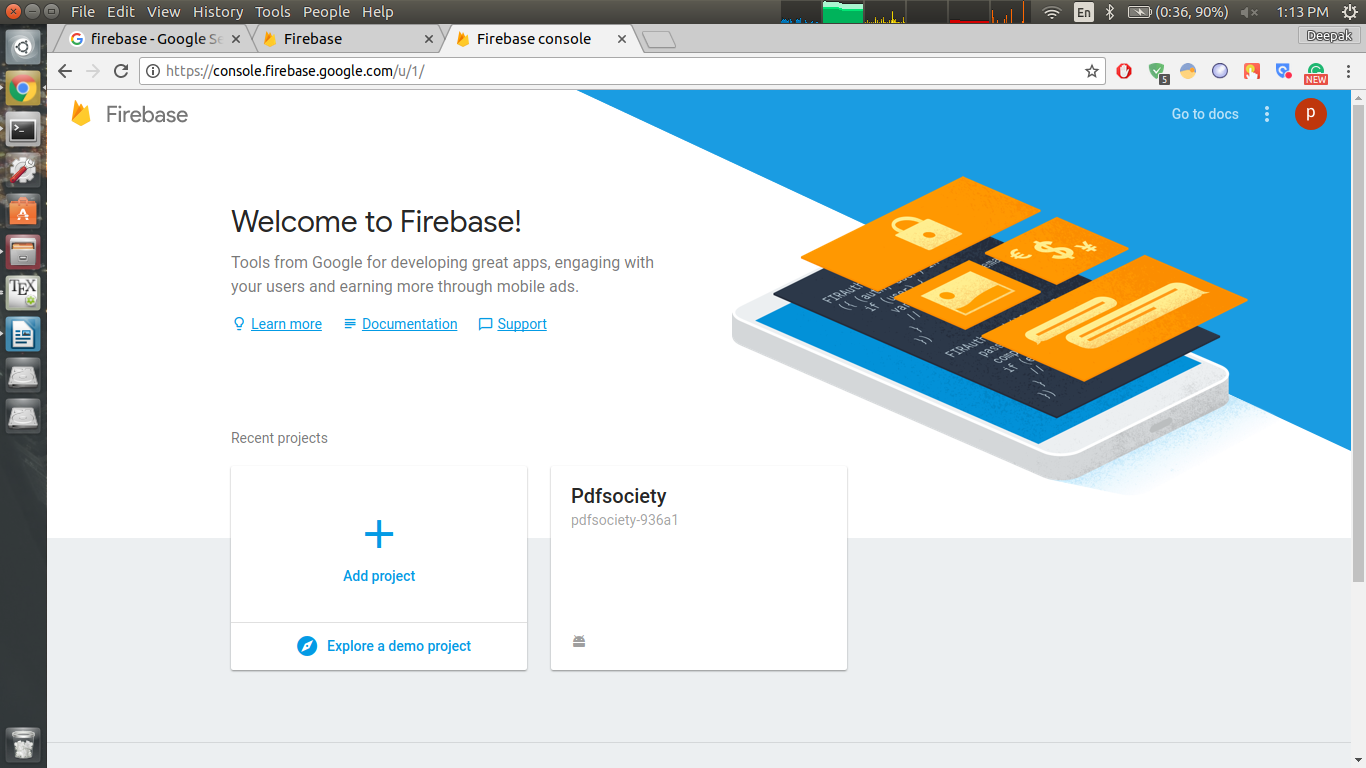
\includegraphics[scale=0.20]{images/Pdf2.png}
\caption{Firebase Console}
\end{figure}

 

\item \textbf{Firebase Products}

\begin{figure}[ht]
\centering
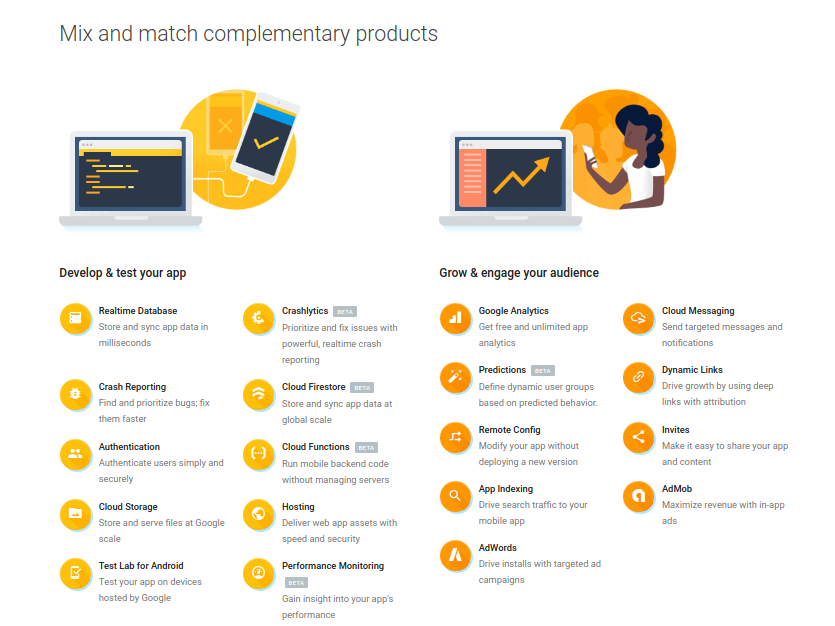
\includegraphics[scale=0.4]{images/Pdf1.png}
\caption{Firebase Products}
\end{figure}

\begin{itemize}

\item \textbf{Firebase Authentication}

Firebase Authentication aims to make building secure authentication systems easy, while improving the sign-in and onboarding experience for end users. It provides an end-to-end identity solution, supporting email and password accounts, phone auth, and Google, Twitter, Facebook, and GitHub login, and more.

Most apps need to know the identity of a user. Knowing a user's identity allows an app to securely save user data in the cloud and provide the same personalized experience across all of the user's devices.
Firebase Authentication provides backend services, easy-to-use SDKs, and ready-made UI libraries to authenticate users to your app. It supports authentication using passwords, phone numbers, popular federated identity providers like Google, Facebook and Twitter, and more.

Firebase Authentication integrates tightly with other Firebase services, and it leverages industry standards like OAuth 2.0 and OpenID Connect, so it can be easily integrated with your custom backend.

\item \textbf{Firebase Realtime Database}

Store and sync data with our NoSQL cloud database. Data is synced across all clients in realtime, and remains available when your app goes offline.

The Firebase Realtime Database is a cloud-hosted database. Data is stored as JSON and synchronized in realtime to every connected client. When you build cross-platform apps with our iOS, Android, and JavaScript SDKs, all of your clients share one Realtime Database instance and automatically receive updates with the newest data.


\item \textbf{Cloud Storage}

Cloud Storage is built for app developers who need to store and serve user-generated content, such as photos or videos.

Cloud Storage for Firebase is a powerful, simple, and cost-effective object storage service built for Google scale. The Firebase SDKs for Cloud Storage add Google security to file uploads and downloads for your Firebase apps, regardless of network quality. You can use our SDKs to store images, audio, video, or other user-generated content. On the server, you can use Google Cloud Storage, to access the same files.
	\end{itemize}
	\end{itemize}
	
\subsubsection{Android}


Android provides a rich application framework that allows you to build innovative
apps and games for mobile devices in a Java language environment. The documents
listed in the left navigation provide details about how to build apps using Android's
various APIs.The various fundamental concepts about the Android app framework:

\begin{figure}[ht]
\centering
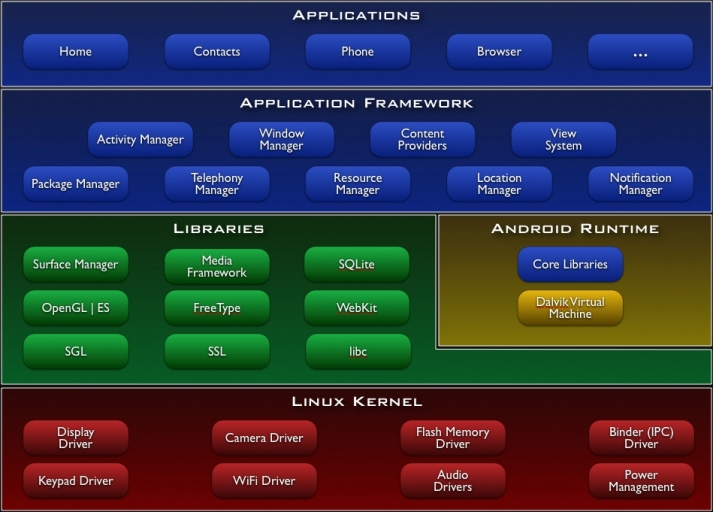
\includegraphics[scale=0.38]{images/a1.jpg}
\caption{Android Anatomy}
\label{fig:Anatomy}
\end{figure}

Apps provide multiple entry points.Android apps are built as a combination of distinct components that can be invoked individually. For instance, an individual activity provides a single screen for a userinterface, and a service independently performs work in the background. From one component you can start another component using an intent. You can even start a component in a different app, such as an activity in a maps app to show an
address. This model provides multiple entry points for a single app and allows any
app to behave as a user's "default" for an action that other apps may invoke.

Apps adapt to different devices, Android provides an adaptive app framework that allows you to provide unique resources for different device configurations. For example, you can create different XML layout les for different screen sizes and the system determines which layout
to apply based on the current device's screen size. You can query the availability of device features at runtime if any app features require specific hardware such as
a camera. If necessary, you can also declare features your app requires so app markets such as Google Play Store do not allow installation on devices that do not
support that feature Android comes with an Android market which is an online
software store. It was developed by Google.

 It allows Android users to select, and
download applications developed by third party developers and use them. There
are around 2.0 lack+ games, application and widgets available on the market for
users. Android applications are written in java programming language. Android is
available as open source for developers to develop applications which can be
further used for selling in android market. There are around 200000 applications
developed for android with over 3 billion+ downloads. Android relies on Linux version 2.6 for core system services such as security, memory management, process management, network stack, and driver model. For software development, Android provides Android SDK (Software development kit).

\begin{itemize}

\item \textbf{Activity Lifecycle}
Activities in the system are managed as an activity stack. When a new activity
is started, it is placed on the top of the stack and becomes the running activitythe previous activity always remains below it in the stack, and will not come to
the foreground again until the new activity exits. An activity has essentially four
states:
If an activity in the foreground of the screen (at the top of the stack), it is
active or running.

If an activity has lost focus but is still visible (that is, a new non-full-sized or
transparent activity has focus on top of your activity), it is paused. A paused
activity is completely alive (it maintains all state and member information and
remains attached to the window manager), but can be killed by the system in
extreme low memory situations.
\begin{figure}[ht]
\centering
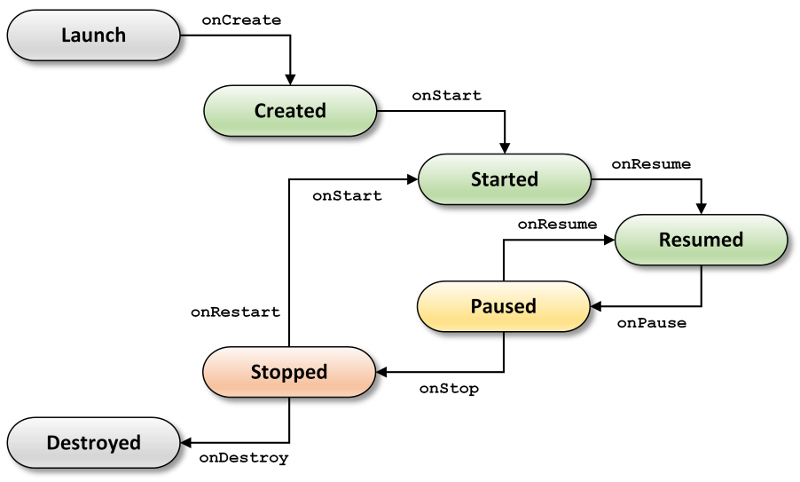
\includegraphics[scale=0.5]{images/a2.png}
\caption{Activity Life Cycle}
\label{fig: Activity }
\end{figure}

If an activity is completely obscured by another activity, it is stopped. It still
retains all state and member information, however, it is no longer visible to
the user so its window is hidden and it will often be killed by the system when
memory is needed elsewhere.

If an activity is paused or stopped, the system can drop the activity from memory by either asking it to finish, or simply killing its process. When it is displayed again to the user, it must be completely restarted and restored to its previous state.


\item \textbf{Libraries used in making this application}

\begin{itemize}
	\item \textbf{Android Support Library}
Android Support Library, Card View, Recycler View, Material : The application will
follow Material design guidelines.

\end{itemize}

\end{itemize}

\subsection{Language used}
\subsubsection{JAVA}

Java is a platform-independent programming language used to create secure
and robust application that may run on a single computer or may be distributed
among servers and clients over a network.

Java features such as platform-independency and portability ensure that while
de-veloping Java EE enterprise applications, you do not face the problems
related to hardware , network , and the operating system.

Java was started as a project called "Oak" by James Gosling in June 1991.
Gosling's goals were to implement a virtual machine and a language that had a
familiar C like notation but with greater uniformity and simplicity than C/C++.
The First publication of Java 1.0 was released by Sun Microsystems in 1995. It
made the promise of "Write Once, Run Anywhere", with free runtimes on
popular platforms. In 2006-2007 Sun released java as open source and
andplateform independent soft-ware. Over time new enhanced versions of Java
have been released. The current version of Java is Java 1.7 which is also
known as Java 7.he Java virtual machine (JVM) is a software implementation of
a computer that executes programs like a real machine. The Java virtual
machine is written specifically for a specific operating system, e.g. for Linux a
special implementation is required as well as for Windows.

Java programs are compiled by the Java compiler into bytecode. The Java
virtual machine interprets this bytecode and executes the Java program.
The Java runtime environment (JRE) consists of the JVM and the Java class li-
braries and contains the necessary functionality to start Java programs.
The JDK contains in addition the development tools necessary to create Java
pro-grams. The JDK consists therefore of a Java compiler, the Java virtual
machine, and the Java class libraries.

The characteristics and features of java are as follows :

\begin{itemize}
	\item \textbf{Simple}
Simple Java is a simple language because of its various features, Java
Doesn?t Support Pointers , Operator Overloading etc. It doesnt require
unreferenced object because java support automatic garbage collection.
Java provides bug free system due to the strong memory management.

\item \textbf{OOPS}
Object-Oriented Programming Language (OOPs) is the
methodology which provide software development and maintenance by
using
object
state,
behavior
Programming Lan-guage
must
,
and
have
properties.
the
Object Oriented following characteristics.
\begin{itemize}
	\item Encapsulation
\item Polymor-phism
 \item Inheritance
\item Abstraction

\end{itemize}
As the languages like Objective C, C++ fullls the above four characteristics yet
they are not fully object oriented lan-guages because they are structured
as well as object oriented languages.In java everything is an Object. Java
can be easily extended since it is based on the Object model.
\item \textbf{Secure}
Secure Java is Secure Language because of its many features it enables to
develop virus-free, tamper-free systems. Authentication techniques are
based on public-key encryption. Java does not support pointer explicitly for
the memory. All Program Run under the sandbox.

\item \textbf{Robust}
Robust Java was created as a strongly typed language. Data type issues
and problems are resolved at compile-time, and implicit casts of a variable
from one type to another are not allowed.
\item \textbf{Platform-independent}
Platform-independent Java Language is platform-independent due to its
hardware and software environment. Java code can be run on multiple
plat-forms e.g. windows, Linux, sun Solaris, Mac/Os etc. Java code is
compiled by the compiler and converted into byte code. This byte code is a
platform independent code because it can be run on multiple platforms i.e.
Write Once and Run Anywhere(WORA).
\item \textbf{Architectural Neural}
Architecture neutral It is not easy to write an application that can be used
on Windows , UNIX and a Macintosh. And its getting more complicated
with the move of windows to non Intel CPU architectures.
Java takes a diffierent approach. Because the Java compiler creates byte
code instructions that are subsequently interpreted by the java interpreter,
archi-tecture neutrality is achieved in the implementation of the java
interpreter for each new architecture.
\item \textbf{Portable}
Portable Java code is portable. It was an important design goal of Java that it
be portable so that as new architectures(due to hardware, operating system,
or both) are developed, the java environment could be ported to them.
In java, all primitive types(integers, longs, oats, doubles, and so on) are
20of de ned sizes, regardless of the machine or operating system on which
the program is run. This is in direct contrast to languages like C and C++
that leave the sized of primitive types up to the compiler and developer.
Additionally, Java is portable because the compiler itself is written in Java.
\item \textbf{Dynamic}
Dynamic Because it is interpreted , Java is an extremely dynamic language, At
runtime, the java environment can extends itself by linking in classes that may
be located on remote servers on a network(for example, the internet)
At runtime, the java interpreter performs name resolution while linking in the
necessary classes. The Java interpreter is also responsible for determining
the placement of object in memory. These two features of the Java interpreter
solve the problem of changing the de nition of a class used by other classes.
\item \textbf{Interpreted}
We all know that Java is an interpreted language as well. With
an interpreted language such as Java, programs run directly from the
source code.
The interpreter program reads the source code and translates it on the y
into computations. Thus, Java as an interpreted language depends on an
interpreter program.
The versatility of being platform independent makes Java to outshine from
other languages. The source code to be written and distributed is platform
independent.
Another advantage of Java as an interpreted language is its error
debugging quality. Due to this any error occurring in the program gets
traced. This is how it is di erent to work with Java.
\item \textbf{High performance}
High performance For all but the simplest or most infrequently used appli-cations,
performance is always a consideration for most applications, including
21graphics-intensive ones such as are commonly found on the world wide web,
the performance of java is more than adequate.
\item \textbf{Multithreading}
Writing a computer program that only does a single thing at a
time is an artificial constraint that lived with in most programming
languages. With java, we no longer have to live with this limitation. Support
for multiple, synchronized threads is built directly into the Java language
and runtime environment. Synchronized threads are extremely useful in
creating distributed, network-aware applications. Such as application may
be commu-nicating with a remote server in one thread while interacting
with a user in a different thread.
\item \textbf{Distributed}
Java facilitates the building of distributed application by a collection
of classes for use in networked applications. By using javas URL (Uniform
Resource Locator) class, an application can easily access a remote server.
Classes also are provided for establishing socket-level connections.


\end{itemize}

\subsubsection{XML}
Extensible Markup Language (XML) is a markup language that defines a set of rules for encoding documents in a format that is both human-readable and machine-readable through use of tags that can be created and defined by users. Much like natural language is extensible (that is, can grow) when speakers create new words and agree on what they mean, XML is a markup language that can grow when users create new elements and agree on what they mean. For example, XML can markup machine-readably that apples and bananas are types of fruit, which is semantically deeper than the purpose of HTML. However, HTML is useful for display of content; often HTML is used to display XML content after transformation with XSL.

\subsection{IDE used}
\subsubsection{Android Studio}

\begin{figure}[ht]
\centering

\includegraphics[scale=0.38]{images/android.png}
\caption{Android Studio}
\end{figure}

Android Studio is the official integrated development environment (IDE) for Google's Android operating system, built on JetBrains' IntelliJ IDEA software and designed specifically for Android development.
It is available for download on Windows, macOS and Linux based operating systems. It is a replacement for the Eclipse Android Development Tools (ADT) as primary IDE for native Android application development. 

Android Studio was announced on May 16, 2013 at the Google I/O conference. It was in early access preview stage starting from version 0.1 in May 2013, then entered beta stage starting from version 0.8 which was released in June 2014. The first stable build was released in December 2014, starting from version 1.0. The current stable version is 2.3.3, released in June 2017. Next major update, version 3.0, is in preview stage as of September 2017.

It offer tools custom-tailored for Android developers, including rich code editing, debugging, testing, and profiling tools.




\begin{itemize}
\item \textbf{System Requirements}
Android application development on either of the following operating systems −
\vskip 0.1in

Microsoft Windows 10/8/7/Vista/2003 (32 or 64-bit)
\\Mac OS X 10.8.5 or higher, up to 10.9 (Mavericks)
\\GNOME or KDE desktop
\vskip 0.1in

Second point is that all the required tools to develop Android applications are open source and can be downloaded from the Web. Following is the list of software's you will need before you start your Android application programming.\\

Java JDK5 or later version
\\Java Runtime Environment (JRE) 6
\\Android Studio
\end{itemize}

\subsection{Introduction to \LaTeX}
\begin{figure}[ht]
\centering
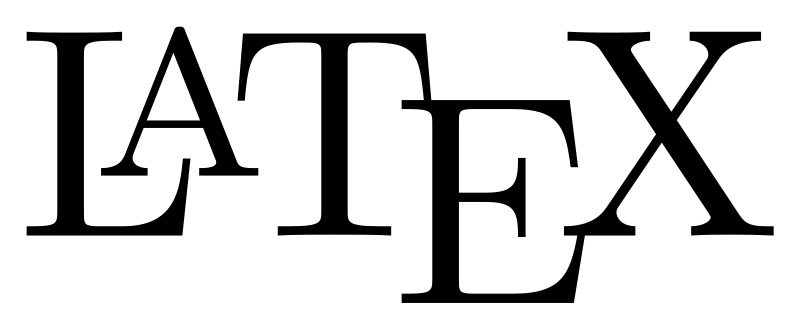
\includegraphics[scale=0.2]{images/latex.png}
\caption{\LaTeX{} Logo}
\end{figure}
\hspace{-1.8em} \LaTeX{}, I had never heard about this term before doing this project,
but when I came to know about it's features, it is just excellent. 
\LaTeX (pronounced /ˈleɪtɛk/, /ˈleɪtɛx/, /ˈlɑːtɛx/, or /ˈlɑːtɛk/) is a 
document markup language and document preparation system for the \TeX{} 
typesetting  program. Within the typesetting system, its name is styled 
as \LaTeX.

\hspace{-1.8em} Within the typesetting system, its name is styled as \LaTeX. The term 
\LaTeX{} refers only to the language in which documents are written, 
not to the editor used to write those documents. In order to create a 
document in \LaTeX, a .tex file must be created using some form of text 
editor. While most text editors can be used to create a \LaTeX{} document, 
a number of editors have been created specifically for working with \LaTeX.\\

\noindent\LaTeX{} is most widely used by mathematicians, scientists, 
engineers, philosophers, linguists, economists and other scholars in 
academia. As a primary or intermediate format, e.g., translating DocBook 
and other XML-based formats to PDF, \LaTeX{} is used because of the 
high quality of typesetting achievable by \TeX. The typesetting system 
offers programmable desktop publishing features and extensive facilities 
for automating most aspects of typesetting and desktop publishing, 
including numbering and cross-referencing, tables and figures, 
page layout and bibliographies.\\

\noindent\LaTeX{} is intended to provide a high-level language that
accesses the power of \TeX. \LaTeX{} essentially comprises a
collection of \TeX{} macros and a program to process \LaTeX documents. 
Because the \TeX{} formatting commands are very low-level, it is usually 
much simpler for end-users to use \LaTeX{}.


\subsubsection{Typesetting}
\LaTeX{} is based on the idea that authors should be able to focus on 
the content of what they are writing without being distracted by its 
visual presentation. in preparing a \LaTeX{} document, the author 
specifies the logical structure using familiar concepts such as 
chapter, section, table, figure, etc., and lets the \LaTeX{} system 
worry about the presentation of these structures. it therefore 
encourages the separation of layout from content while still allowing 
manual typesetting adjustments where needed. 

\begin{verbatim}
\documentclass[12pt]{article}
\usepackage{amsmath}
\title{\LaTeX}
\begin{document}
  \maketitle 
  \LaTeX{} is a document preparation system 
  for the \TeX{} typesetting program.
   \par 
   $E=mc^2$
\end{document}
\end{verbatim}

\subsubsection{Installing \LaTeX{} on System}
Installation of \LaTeX{} on personal system is quite easy. As i have used \LaTeX{} on Ubuntu 13.04 so i am discussing the installation steps for Ubuntu 13.04 here:
\begin{itemize}
\item Go to terminal and type\\\\
\textit{sudo apt-get install texlive-full}
\item Your Latex will be installed on your system and you can check for manual page by typing.\\\\
\textit{man latex}\\

in terminal which gives manual for latex command.
\item To do very next step now one should stick this to mind that the document which one is going to produce is written in any type of editor whether it may be your most common usable editor Gedit or you can use vim by installing first vim into your system using command.\\\\
\textit{sudo apt-get install vim}
\item After you have written your document it is to be embedded with some set of commands that Latex uses so as to give a structure to your document. Note that whenever you wish your document to be looked into some other style just change these set of commands.
\item When you have done all these things save your piece of code with .tex format say test.tex. Go to terminal and type\\\\
\textit{latex path of the file test.tex Or pdflatex path of the file test.tex\\ eg: pdflatex test.tex}\\
for producing pdf file simultaneously.\\
After compiling it type command\\\\
\textit{evince filename.pdf\\ eg: evince test.pdf}\\
To see output pdf file. 
\end{itemize}
\subsubsection{Pdfscreen \LaTeX{}}
There are some packages that can help to have unified document using \LaTeX{}. Example of such a package is pdfscreen that let the user view it’s document in two forms-print and screen. Print for hard copy and screen for viewing your document on screen. Download this package from www.ctan.org/tex-archive/macros/latex/contrib/pdfscreen/.\\
Then install it using above mention method.\\

\noindent To test it the test code is given below:-\\
Just changing print to screen gives an entirely different view. But for working of pdfscreen another package required are comment and fancybox.\\

\noindent The fancybox package provides several different styles of boxes for framing and rotating content in your document. Fancybox provides commands that produce square-cornered boxes with single or double lines, boxes with shadows, and round-cornered boxes with normal or bold lines. You can box mathematics, floats, center, flushleft, and flushright, lists, and pages.\\
 	
\noindent Whereas comments package selectively include/excludes portions of text. The comment package allows you to declare areas of a document to be included or excluded. One need to make these declarations in the preamble of your file. The package uses a method for exclusion that is pretty robust, and can cope with ill-formed bunches of text.\\

\noindent So these extra packages needed to be installed on system for the proper working of pdfscreen package.


	\section{Coding standards of Language used 
}

\subsection{Introduction}
This document is the definition of Google's coding standards for source code in the Java Programming Language. A Java source file is described as being in Google Style if and only if it adheres to the rules herein.
Like other programming style guides, the issues covered span not only aesthetic issues of formatting, but other types of conventions or coding standards as well. However, this document focuses primarily on the hard-and-fast rules that we follow universally, and avoids giving advice that isn't clearly enforceable (whether by human or tool).
\subsection{Source file basics}
\begin{itemize}
\item File name, the source file name consists of the case-sensitive name of the top-level class it contains (of which there is exactly one), plus the .java extension.
\item File encoding: UTF-8 Source files are encoded in UTF-8.Aside from the line terminator sequence, the ASCII horizontal space character (0x20) is the only whitespace character that appears anywhere in a source file. This implies that:
\item All other whitespace characters in string and character literals are escaped.
\item Tab characters are not used for indentation.
\end{itemize}

	\section{GANTT chart}
	
	\begin{figure}[ht]
\centering
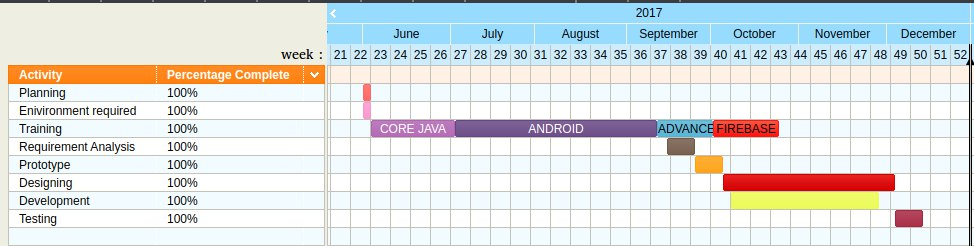
\includegraphics[scale=0.43]{images/gantchart.jpg}
\caption{GANTT chart}
\end{figure}


	\section{Testing Techniques and Test Plans}
	\subsection{Testing Techniques}
	
\subsubsection{xUnit Framework}
xUnit is the collective name for several unit testing frameworks that derive their structure and functionality from Smalltalk's SUnit. SUnit, designed by Kent Beck in 1998, was written in a highly structured object-oriented style, which lent easily to contemporary languages such as Java and C. Following its introduction in Smalltalk the framework was ported to Java by Kent Beck and Erich Gamma and gained wide popularity, eventually gaining ground in the majority of programming languages in current use. The names of many of these frameworks are a variation on "SUnit", usually replacing the "S" with the first letter (or letters) in the name of their intended language ("JUnit" for Java, "RUnit" for R etc.). These frameworks and their common architecture are collectively known as "xUnit".
\subsubsection{JUnit}
JUnit is a unit testing framework for the Java programming language. JUnit has been important in the development of test-driven development, and is one of a family of unit testing frameworks which is collectively known as xUnit that originated with SUnit. JUnit is linked as a JAR at compile-time; the framework resides under package junit.framework for JUnit 3.8 and earlier, and under package org.junit for JUnit 4 and later. A research survey performed in 2013 across 10,000 Java projects hosted on GitHub found that JUnit, (in a tie with slf4j-api), was the most commonly included external library. Each library was used by 30.7 percentage of projects.
\subsubsection{Robotium Android Testing Tool}
Robotium is one the first and frequently utilized automated testing tools for software supported on Android. Robotium is a free Android UI testing tool. It is suitable for tests automation for different Android versions and sub-versions. Software developers often describe it as Selenium for Android. Tests created by Robotium are written in Java. In fact, Robotium is a library for unit tests.
But it takes much time and efforts to create tests by means of Robotium, as one must work with the program source code in order to automate tests. The tool is also unsuitable for interaction with system software; it cannot lock and unlock a smartphone or a tablet. There is no Record and Play function in Robotium, and it does not provide screenshots.
\subsubsection{MonkeyRunner Android App Testing}
MonkeyRunner Android App Testing
MonkeyRunner is one of popular Android Testing tools used for automating of functional tests for Android software. This tool is more low-level than Robotium is. One does not have to deal with the source code in order to automate tests. The tests are written in Python, one may use a recording tool for creating tests.
MonkeyRunner can run tests on real devices connected to a PC or emulators. The tool has an API what allows it to control a smartphone, a tablet or an emulator from outside of Android code. A significant disadvantage of the mobile app testing tool is that it is necessary to write scripts for each device. Another problem of MonkeyRunner is that the tests require adjustments each time when user interface of the tested program is changed.
\newpage
\subsection{Test Plans}

\subsubsection{Testing of login}

\begin{table}[h!]
\centering
\caption{Login test} \vskip0.3cm
\begin{tabular}{ | m{5em} | m{5cm}|} 
\hline
Test Id: & TC1   \\ 
\hline
Tester: & Admin  \\ 
\hline
Date: & 8-11-2017  \\ 
\hline
Purpose: & Login to system   \\ 
\hline
Pre-requisites: & Must fill login form   \\ 
\hline
Test Data: & Email, Password   \\ 
\hline
Steps: &  \\
\hline  
Step 1 &  Start Application \\ 
Step 2 &  Login Activity will be displayed  \\ 
Step 3 &  Enter password  \\ 
Step 4 &  Click login  \\ 
Step 5 &  If the email and password is correct Home Activity will appear  \\ 
Step 6 &  If the username and password is not correct toast will appear \\
\hline
Status: & Pass   \\ 
\hline
\end{tabular}
\label{table:1}
\end{table}

\newpage

\subsubsection{Testing of Uploading Pdf} 	

\begin{table}[h!]
\centering
\caption{Upload pdf test} \vskip0.3cm
\begin{tabular}{ | m{5em} | m{5cm}|} 
\hline
Test Id: & TC2   \\ 
\hline
Tester: & Admin  \\ 
\hline
Date: & 12-11-2017  \\ 
\hline
Purpose: & Uploading Pdf to database   \\ 
\hline
Pre-requisites: & Must be login   \\ 
\hline
Test Data: & Email, Password, Any Pdf   \\ 
\hline
Steps: &  \\
\hline  
Step 1 &  Start Application \\ 
Step 2 &  Login Activity will be displayed  \\ 
Step 3 &  Enter password  \\ 
Step 4 &  Click login  \\ 
Step 5 &  Home Activity will appear  \\ 
Step 6 &  Click on Fab button \\
Step 7 &  Upload Activity open \\
Step 8 &  Choose Pdf to be upload \\
Step 9 &  Enter Description(if not added then error display) \\
Step 10 &  Click on Upload button and it will be uploaded \\
\hline
Status: & Pass   \\ 
\hline
\end{tabular}
\label{table:2}
\end{table}

\newpage


\subsubsection{Testing of Retrieving Pdf database} 	

 \begin{table}[h!]
\centering
\caption{Retrieving pdf test} \vskip0.3cm
\begin{tabular}{ | m{5em} | m{5cm}|} 
\hline
Test Id: & TC3   \\ 
\hline
Tester: & Admin  \\ 
\hline
Date: & 21-11-2017  \\ 
\hline
Purpose: & Retrieving Pdf from database   \\ 
\hline
Pre-requisites: & Must be login and Pdf in database  \\ 
\hline
Test Data: & Email, Password, Any Pdf in database   \\ 
\hline
Steps: &  \\
\hline  
Step 1 &  Start Application \\ 
Step 2 &  Login Activity will be displayed  \\ 
Step 3 &  Enter password  \\ 
Step 4 &  Click login  \\ 
Step 5 &  Home Activity will appear and Pdf displayed in Fragment  \\ 
\hline
Status: & Pass   \\ 
\hline
\end{tabular}
\label{table:3}
\end{table}
\newpage

\subsubsection{Testing of Downloading Pdf} 	

 \begin{table}[h!]
\centering
\caption{Downloading pdf test} \vskip0.3cm
\begin{tabular}{ | m{5em} | m{5cm}|} 
\hline
Test Id: & TC4   \\ 
\hline
Tester: & Admin  \\ 
\hline
Date: & 25-11-2017  \\ 
\hline
Purpose: & Downloading Pdf from database   \\ 
\hline
Pre-requisites: & Must be login and Pdf in database  \\ 
\hline
Test Data: & Email, Password, Pdf    \\ 
\hline
Steps: &  \\
\hline  
Step 1 &  Start Application \\ 
Step 2 &  Login Activity will be displayed  \\ 
Step 3 &  Enter password  \\ 
Step 4 &  Click login  \\ 
Step 5 &  Home Activity will appear  \\ 
Step 6 &  Click on Pdf  \\
Step 7 &  Pdf Detail Activity open \\
Step 8 &  Click on Download button and it will be uploaded \\
Step 9 &  Drag notification bar and open downloaded pdf \\ 
\hline
Status: & Pass   \\ 
\hline
\end{tabular}
\label{table:4}
\end{table}
\newpage

\subsubsection{Testing of Uploading Pdf in particular category} 	

\begin{table}[h!]
\centering
\caption{Upload pdf in particular category test} \vskip0.3cm
\begin{tabular}{ | m{5em} | m{5cm}|} 
\hline
Test Id: & TC5   \\ 
\hline
Tester: & Admin  \\ 
\hline
Date: & 30-11-2017  \\ 
\hline
Purpose: & Uploading Pdf into particular category   \\ 
\hline
Pre-requisites: & Must be login   \\ 
\hline
Test Data: & Email, Password, Any Pdf   \\ 
\hline
Steps: &  \\
\hline  
Step 1 &  Start Application \\ 
Step 2 &  Login Activity will be displayed  \\ 
Step 3 &  Enter password  \\ 
Step 4 &  Click login  \\ 
Step 5 &  Home Activity will appear  \\ 
Step 6 &  Click on Fab button \\
Step 7 &  Upload Activity open \\
Step 8 &  Choose Pdf to be upload \\
Step 8 &  Select category of Pdf \\
Step 9 &  Enter Description(if not added then error display) \\
Step 10 &  Click on Upload button and it will be uploaded in that category \\
\hline
Status: & Pass   \\ 
\hline
\end{tabular}
\label{table:5}
\end{table}
\newpage

\subsubsection{Testing of sharing pdf to various app} 	

 \begin{table}[h!]
\centering
\caption{Share ebook test} \vskip0.3cm
\begin{tabular}{ | m{5em} | m{5cm}|} 
\hline
Test Id: & TC6   \\ 
\hline
Tester: & Admin  \\ 
\hline
Date: & 2-12-2017  \\ 
\hline
Purpose: & Sharing pdf to various app   \\ 
\hline
Pre-requisites: & Must be login and pdf for sharing   \\ 
\hline
Test Data: & Email, Password, Any Pdf   \\ 
\hline
Steps: &  \\
\hline  
Step 1 &  Start Application \\ 
Step 2 &  Login Activity will be displayed  \\ 
Step 3 &  Enter password  \\ 
Step 4 &  Click login  \\ 
Step 5 &  Home Activity will appear  \\ 
Step 6 &  Click on Pdf  \\
Step 7 &  Pdf Detail Activity open \\
Step 8 &  Select share icon from menu \\
Step 9 &  Choose apps for sharing pdf \\
\hline
Status: & Pass   \\ 
\hline
\end{tabular}
\label{table:6}
\end{table}
 
 
 
 
